\documentclass[journal,12pt,twocolumn]{IEEEtran}

\usepackage{setspace}
\usepackage{gensymb}
\singlespacing
\usepackage[cmex10]{amsmath}

\usepackage{amsthm}

\usepackage{mathrsfs}
\usepackage{txfonts}
\usepackage{stfloats}
\usepackage{bm}
\usepackage{cite}
\usepackage{cases}
\usepackage{subfig}

\usepackage{longtable}
\usepackage{multirow}

\usepackage{enumitem}
\usepackage{mathtools}
\usepackage{steinmetz}
\usepackage{tikz}
\usepackage{circuitikz}
\usepackage{verbatim}
\usepackage{tfrupee}
\usepackage[breaklinks=true]{hyperref}
\usepackage{graphicx}
\usepackage{tkz-euclide}

\usetikzlibrary{calc,math}
\usepackage{listings}
    \usepackage{color}                                            %%
    \usepackage{array}                                            %%
    \usepackage{longtable}                                        %%
    \usepackage{calc}                                             %%
    \usepackage{multirow}                                         %%
    \usepackage{hhline}                                           %%
    \usepackage{ifthen}                                           %%
    \usepackage{lscape}     
\usepackage{multicol}
\usepackage{chngcntr}

\DeclareMathOperator*{\Res}{Res}

\renewcommand\thesection{\arabic{section}}
\renewcommand\thesubsection{\thesection.\arabic{subsection}}
\renewcommand\thesubsubsection{\thesubsection.\arabic{subsubsection}}

\renewcommand\thesectiondis{\arabic{section}}
\renewcommand\thesubsectiondis{\thesectiondis.\arabic{subsection}}
\renewcommand\thesubsubsectiondis{\thesubsectiondis.\arabic{subsubsection}}


\hyphenation{op-tical net-works semi-conduc-tor}
\def\inputGnumericTable{}                                 %%

\lstset{
%language=C,
frame=single, 
breaklines=true,
columns=fullflexible
}
\begin{document}


\newtheorem{theorem}{Theorem}[section]
\newtheorem{problem}{Problem}
\newtheorem{proposition}{Proposition}[section]
\newtheorem{lemma}{Lemma}[section]
\newtheorem{corollary}[theorem]{Corollary}
\newtheorem{example}{Example}[section]
\newtheorem{definition}[problem]{Definition}

\newcommand{\BEQA}{\begin{eqnarray}}
\newcommand{\EEQA}{\end{eqnarray}}
\newcommand{\define}{\stackrel{\triangle}{=}}
\bibliographystyle{IEEEtran}
\raggedbottom
\setlength{\parindent}{0pt}
\providecommand{\mbf}{\mathbf}
\providecommand{\pr}[1]{\ensuremath{\Pr\left(#1\right)}}
\providecommand{\qfunc}[1]{\ensuremath{Q\left(#1\right)}}
\providecommand{\sbrak}[1]{\ensuremath{{}\left[#1\right]}}
\providecommand{\lsbrak}[1]{\ensuremath{{}\left[#1\right.}}
\providecommand{\rsbrak}[1]{\ensuremath{{}\left.#1\right]}}
\providecommand{\brak}[1]{\ensuremath{\left(#1\right)}}
\providecommand{\lbrak}[1]{\ensuremath{\left(#1\right.}}
\providecommand{\rbrak}[1]{\ensuremath{\left.#1\right)}}
\providecommand{\cbrak}[1]{\ensuremath{\left\{#1\right\}}}
\providecommand{\lcbrak}[1]{\ensuremath{\left\{#1\right.}}
\providecommand{\rcbrak}[1]{\ensuremath{\left.#1\right\}}}
\theoremstyle{remark}
\newtheorem{rem}{Remark}
\newcommand{\sgn}{\mathop{\mathrm{sgn}}}
\providecommand{\abs}[1]{\left\vert#1\right\vert}
\providecommand{\res}[1]{\Res\displaylimits_{#1}} 
\providecommand{\norm}[1]{\left\lVert#1\right\rVert}
%\providecommand{\norm}[1]{\lVert#1\rVert}
\providecommand{\mtx}[1]{\mathbf{#1}}
\providecommand{\mean}[1]{E\left[ #1 \right]}
\providecommand{\fourier}{\overset{\mathcal{F}}{ \rightleftharpoons}}
%\providecommand{\hilbert}{\overset{\mathcal{H}}{ \rightleftharpoons}}
\providecommand{\system}{\overset{\mathcal{H}}{ \longleftrightarrow}}
	%\newcommand{\solution}[2]{\textbf{Solution:}{#1}}
\newcommand{\solution}{\noindent \textbf{Solution: }}
\newcommand{\cosec}{\,\text{cosec}\,}
\providecommand{\dec}[2]{\ensuremath{\overset{#1}{\underset{#2}{\gtrless}}}}
\newcommand{\myvec}[1]{\ensuremath{\begin{pmatrix}#1\end{pmatrix}}}
\newcommand{\mydet}[1]{\ensuremath{\begin{vmatrix}#1\end{vmatrix}}}
\numberwithin{equation}{subsection}
\makeatletter
\@addtoreset{figure}{problem}
\makeatother
\let\StandardTheFigure\thefigure
\let\vec\mathbf
\renewcommand{\thefigure}{\theproblem}
\def\putbox#1#2#3{\makebox[0in][l]{\makebox[#1][l]{}\raisebox{\baselineskip}[0in][0in]{\raisebox{#2}[0in][0in]{#3}}}}
     \def\rightbox#1{\makebox[0in][r]{#1}}
     \def\centbox#1{\makebox[0in]{#1}}
     \def\topbox#1{\raisebox{-\baselineskip}[0in][0in]{#1}}
     \def\midbox#1{\raisebox{-0.5\baselineskip}[0in][0in]{#1}}
\vspace{3cm}
\title{AI5002: Assignment 13}
\author{Debolena Basak\\ AI20RESCH11003}
\maketitle
\newpage
\bigskip
\renewcommand{\thefigure}{\theenumi}
\renewcommand{\thetable}{\theenumi}
Download all Python codes from 
\begin{lstlisting}
https://github.com/Debolena/AI5002-Probability-and-Random-Variables/blob/main/Assignment_13/simulation%20code.py
\end{lstlisting}
%
and latex-tikz codes from 
%
\begin{lstlisting}
https://github.com/Debolena/AI5002-Probability-and-Random-Variables/blob/main/Assignment_13/latex_code.tex
\end{lstlisting}
\section{Problem}
A random variable $X$ has probability density
function $f(x)$ as given below:
\begin{align}
    f\brak x = 
    \begin{cases}
    a + bx  , \quad 0<x<1 \\
    0, \quad otherwise \label{fx}
    \end{cases}
\end{align}
If the expected value $E[X] = \frac{2}{3}$, then $Pr[X<0.5]$ is..........
\section{Solution}
First, we need to find out the values of a and b.\\
We know,
\begin{align}
    & \int_{-\infty}^{\infty} f\brak x dx =1\\
    &\implies \int_0^1 \brak{a+bx} \; dx = 1\\
    &\implies \sbrak {ax + b\frac{x^2}{2}}_0^1 = 1\\
    &\implies a + \frac{b}{2} = 1\\
    &\implies 2a +b = 2 \label{eq1}
\end{align}
\begin{align}
    & \quad \quad E\brak X = \frac{2}{3}\\
    &\implies \int_0^1 x f\brak x dx = \frac{2}{3} \\
    &\implies \int_0^1 x\brak{a + bx} dx = \frac{2}{3}\\
    &\implies \sbrak{a\frac{x^2}{2}+ b\frac{x^3}{3}}_0^1 = \frac{2}{3}\\
    &\implies{\frac{a}{2}+ \frac{b}{3}} = \frac{2}{3}\\
    &\implies 3a + 2b = 4 \label{eq2}
\end{align}
Multiplying \eqref{eq1} with 2 and subtracting \eqref{eq2} from it, we get
\begin{align}
    a = 0\label{eq: a}
\end{align}
Putting \eqref{eq: a} in \eqref{eq1}, we get
\begin{align}
     b=2 \label{eq: b}
\end{align}
Using \eqref{eq: a} and \eqref{eq: b} in \eqref{fx},
\begin{align}
    f\brak x  = 
    \begin{cases}
    2x  , \quad 0<x<1 \\
    0, \quad otherwise
    \end{cases}
\end{align}
\begin{align}
    \therefore Pr\brak{X<0.5} &= \int_0^{0.5} f\brak x dx\\ 
    &= \int_0^{0.5} 2x \; dx\\
    & = 2\sbrak{\frac{x^2}{2}}_0^{0.5} = \brak{0.5}^2\\
    &= 0.25
\end{align}
\begin{figure}[!ht]
\centering
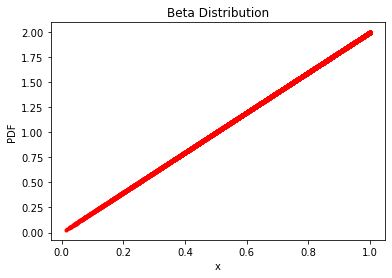
\includegraphics[width=\columnwidth]{pdf plot.png}
\caption{Beta Distribution Plot}
\label{fig:Beta Plot}
\end{figure}
\end{document}
